\section{Kiến trúc Build System trong Yocto Project}
\begin{figure}[H]
    \centering
    
\includegraphics[width=0.4\textwidth]{image/yocto_prj.png}
    \caption{Yocto Project}
    \label{fig:yocto}
\end{figure}

\subsection{Các thành phần chính trong Layer của Yocto Project}

Trong Yocto Project, kiến trúc layer được xây dựng dựa trên cơ chế metadata nhằm tổ chức hệ thống build theo hướng module hóa và có khả năng mở rộng cao. Mỗi layer đóng vai trò như một đơn vị chức năng độc lập, có thể chứa đầy đủ các thành phần cần thiết để xây dựng phần mềm hoặc hệ thống Linux nhúng. Việc phân chia các thành phần trong layer giúp quá trình phát triển, bảo trì và tái sử dụng mã nguồn trở nên thuận tiện hơn. Các thành phần chính thường xuất hiện trong một layer bao gồm Recipe, Configuration, Patch và Source Code.

\subsubsection{Recipe (.bb)}

Recipe là thành phần cốt lõi trong Yocto Project, được sử dụng để mô tả toàn bộ quy trình xây dựng một package hoặc một thành phần phần mềm trong hệ thống nhúng. Các recipe thường có phần mở rộng \texttt{.bb} và được xử lý bởi BitBake Build Engine. Có thể xem recipe như một tập hợp metadata dùng để hướng dẫn hệ thống build thực hiện các công việc như tải mã nguồn, giải nén, biên dịch, cài đặt và đóng gói phần mềm. 

Trong mỗi recipe, nhiều biến hệ thống được sử dụng để mô tả thông tin liên quan đến package. Các biến này bao gồm tên package, phiên bản, giấy phép sử dụng, dependency, vị trí source code và các task cần thực hiện trong quá trình build. Thông qua recipe, BitBake có thể tự động phân tích dependency giữa các package và xây dựng quy trình biên dịch phù hợp.

\subsubsection{Configuration}

Configuration là thành phần chịu trách nhiệm quản lý và thiết lập môi trường build trong Yocto Project. Các file cấu hình thường được lưu trong thư mục \texttt{conf/} và chứa các biến hệ thống phục vụ quá trình xây dựng Linux Embedded. Đây là thành phần quan trọng giúp xác định cách thức hoạt động của toàn bộ hệ thống build. Thông qua configuration, người phát triển có thể thiết lập kiến trúc phần cứng mục tiêu, compiler, toolchain, package manager, loại filesystem và nhiều tham số hệ thống khác. Ngoài ra, configuration còn cho phép quản lý danh sách layer được sử dụng trong môi trường build cũng như thứ tự ưu tiên giữa các layer.

\subsubsection{Patch}

Patch là thành phần được sử dụng để sửa đổi hoặc cập nhật mã nguồn trong quá trình build mà không cần thay đổi trực tiếp source code gốc. Trong Yocto Project, patch đóng vai trò quan trọng trong việc tùy biến phần mềm, sửa lỗi hệ thống và bổ sung chức năng mới cho các package. Patch thường được lưu dưới dạng file \texttt{.patch} hoặc \texttt{.diff}. Các file này chứa thông tin thay đổi giữa phiên bản mã nguồn gốc và phiên bản đã được chỉnh sửa. Trong quá trình build, BitBake sẽ tự động áp dụng patch trước khi thực hiện biên dịch mã nguồn.

\subsubsection{Source Code}

Source Code là thành phần chứa mã nguồn của chương trình hoặc hệ thống phần mềm được sử dụng trong quá trình build. Đây là thành phần cốt lõi quyết định chức năng và hành vi của package trong hệ thống Linux Embedded. Trong Yocto Project, source code có thể được lấy từ nhiều nguồn khác nhau như local file, Git repository, tarball package hoặc remote server. Hệ thống BitBake sẽ tự động tải và quản lý source code dựa trên thông tin được khai báo trong recipe. Source code trong hệ thống nhúng thường bao gồm nhiều loại thành phần như application, library, kernel module, bootloader hoặc device driver. Tùy thuộc vào chức năng của package, source code có thể được viết bằng các ngôn ngữ như C, C++, Python hoặc Shell Script.

\subsection{Recipe trong Yocto}

Trong Yocto Project, Recipe là thành phần trung tâm của hệ thống build và đóng vai trò mô tả toàn bộ quy trình xây dựng một package phần mềm. Recipe thường có phần mở rộng \texttt{.bb} (BitBake Recipe) và được BitBake sử dụng để thực hiện các tác vụ như tải mã nguồn, cấu hình môi trường build, biên dịch, cài đặt và đóng gói package.\cite{yocto_new_recipe} 

Có thể xem recipe như một tập hợp metadata dùng để hướng dẫn BitBake cách xây dựng một thành phần phần mềm cụ thể trong hệ thống Linux Embedded. Thông qua recipe, Yocto Project có khả năng tự động hóa toàn bộ quy trình build và quản lý dependency giữa các package trong hệ thống. Một recipe thường chứa nhiều biến và task nhằm mô tả thông tin liên quan đến package. Các biến này được sử dụng để khai báo metadata như tên package, phiên bản, license, vị trí source code và phương thức build. Trong khi đó, các task chịu trách nhiệm thực thi từng giai đoạn trong pipeline build của BitBake. 

Một số biến quan trọng trong recipe được trình bày trong Bảng \ref{tab:recipe_variables}.

\begin{table}[H]
\centering


\begin{tabular}{|c|p{9cm}|}
\hline
\textbf{Biến} & \textbf{Ý nghĩa} \\ \hline

\texttt{SUMMARY} &
Mô tả ngắn gọn chức năng hoặc mục đích của package. \\ \hline

\texttt{DESCRIPTION} &
Mô tả chi tiết hơn về package và chức năng của phần mềm. \\ \hline

\texttt{LICENSE} &
Khai báo license của package nhằm phục vụ quản lý bản quyền phần mềm. \\ \hline

\texttt{SRC\_URI} &
Khai báo đường dẫn source code hoặc patch được sử dụng trong quá trình build. \\ \hline

\texttt{S} &
Xác định thư mục chứa source code sau khi giải nén. \\ \hline

\texttt{DEPENDS} &
Khai báo các package phụ thuộc cần thiết trước khi build package hiện tại. \\ \hline

\texttt{RDEPENDS} &
Khai báo dependency cần thiết khi package chạy trên hệ thống đích. \\ \hline

\texttt{inherit} &
Kế thừa các class của Yocto nhằm bổ sung chức năng build cho recipe. \\ \hline

\texttt{do\_compile} &
Task dùng để biên dịch source code thành binary executable hoặc kernel module. \\ \hline

\texttt{do\_install} &
Task dùng để cài đặt các file output vào root filesystem tạm thời. \\ \hline

\end{tabular}
\caption{Các biến cơ bản trong Recipe}
\label{tab:recipe_variables}
\end{table}

Trong quá trình build, BitBake sẽ phân tích dependency giữa các recipe để xác định thứ tự thực thi phù hợp. Nhờ đó, hệ thống có thể tự động build toàn bộ Linux Embedded Image với số lượng package lớn mà vẫn đảm bảo tính nhất quán.

\subsection{BitBake Build Engine}

BitBake là build engine trung tâm của Yocto Project, chịu trách nhiệm phân tích metadata và thực thi các task được định nghĩa trong recipe nhằm xây dựng package hoặc toàn bộ hệ thống Linux Embedded. Có thể xem BitBake như một hệ thống tự động hóa build hoạt động dựa trên metadata, cho phép quản lý dependency, thực thi pipeline build và tạo ra image Linux hoàn chỉnh cho nền tảng nhúng.

Trong Yocto Project, mỗi recipe sẽ được BitBake phân tích để xác định các task cần thực hiện cũng như mối quan hệ phụ thuộc giữa các package. Dựa trên dependency graph, BitBake sẽ tự động xác định thứ tự thực thi phù hợp nhằm đảm bảo quá trình build diễn ra chính xác và nhất quán.

Một trong những ưu điểm quan trọng của BitBake là khả năng tự động hóa toàn bộ quá trình build. Thay vì thực hiện thủ công từng bước như tải source code, cấu hình compiler hoặc cài đặt package, BitBake cho phép toàn bộ pipeline build được mô tả thông qua metadata trong recipe. Điều này giúp giảm đáng kể độ phức tạp trong quá trình phát triển hệ thống Linux Embedded.

Các task chính của BitBake được trình bày trong Bảng \ref{tab:bitbake_tasks}.

\begin{table}[H]
\centering
\begin{tabular}{|c|l|}
\hline
\textbf{Task} & \textbf{Chức năng} \\ \hline
do\_fetch & Tải source code \\ \hline
do\_unpack & Giải nén source \\ \hline
do\_patch & Áp dụng patch \\ \hline
do\_compile & Biên dịch mã nguồn \\ \hline
do\_install & Cài đặt package \\ \hline
do\_package & Đóng gói package \\ \hline
\end{tabular}
\caption{Các task chính của BitBake}
\label{tab:bitbake_tasks}
\end{table}

\noindent \textbf{Task do\_fetch}

Task \texttt{do\_fetch} là giai đoạn đầu tiên trong pipeline build của BitBake, chịu trách nhiệm tải source code và các tài nguyên cần thiết cho quá trình build. Dữ liệu có thể được lấy từ Git repository, HTTP server, FTP server, local file hoặc tarball package thông qua biến \texttt{SRC\_URI}.

\noindent \textbf{Task do\_unpack}

Sau khi tải source code, BitBake thực hiện task \texttt{do\_unpack} để giải nén và chuẩn bị mã nguồn cho các bước xử lý tiếp theo. Các file như \texttt{.tar.gz}, \texttt{.zip} hoặc source package sẽ được giải nén vào thư mục làm việc của BitBake, đồng thời source code từ Git repository sẽ được checkout vào workspace tương ứng.

\noindent \textbf{Task do\_patch}

Task \texttt{do\_patch} được sử dụng để áp dụng patch lên source code sau khi giải nén hoàn tất. Cơ chế này cho phép sửa lỗi phần mềm, tùy biến kernel hoặc driver, bổ sung tính năng mới và tối ưu hệ thống cho phần cứng mục tiêu mà không cần thay đổi trực tiếp source code gốc.

\noindent \textbf{Task do\_compile}

Task \texttt{do\_compile} chịu trách nhiệm biên dịch source code thành binary executable cho hệ thống đích. Trong Linux Embedded, quá trình này sử dụng cross-compiler để tạo binary phù hợp với các kiến trúc như ARM, x86 hoặc RISC-V. BitBake sẽ tự động cấu hình compiler, sysroot và môi trường build dựa trên metadata của hệ thống. Task này hỗ trợ build application, library, kernel module và Linux Kernel.

\noindent \textbf{Task do\_install}

Sau khi biên dịch hoàn tất, BitBake thực hiện task \texttt{do\_install} để cài đặt các file output vào thư mục staging hoặc root filesystem tạm thời. Trong giai đoạn này, các binary, library và configuration file sẽ được sắp xếp theo đúng cấu trúc filesystem của Linux nhằm phục vụ quá trình tạo image hệ thống.

\noindent\textbf{Task do\_package}

Task \texttt{do\_package} là giai đoạn cuối trong pipeline build của BitBake, chịu trách nhiệm đóng gói các file đã cài đặt thành package triển khai trên hệ thống đích. BitBake hỗ trợ nhiều định dạng package như \texttt{RPM}, \texttt{DEB} và \texttt{IPK}.

\subsection{Cross-compilation trong Yocto}

Trong các hệ thống Linux Embedded, kiến trúc phần cứng của thiết bị đích thường khác với kiến trúc của máy tính dùng để phát triển phần mềm. Do đó, quá trình biên dịch mã nguồn không thể thực hiện trực tiếp bằng compiler thông thường trên hệ thống host. Để giải quyết vấn đề này, Yocto Project sử dụng cơ chế Cross-compilation nhằm hỗ trợ biên dịch phần mềm cho nhiều nền tảng phần cứng khác nhau.

Cross-compilation là quá trình biên dịch mã nguồn trên một hệ thống máy tính nhưng chương trình được tạo ra sẽ chạy trên một hệ thống khác có kiến trúc phần cứng khác biệt. Trong Linux Embedded, quá trình này thường diễn ra khi source code được build trên máy tính x86 nhưng binary output được thiết kế để chạy trên thiết bị ARM, RISC-V hoặc các nền tảng nhúng chuyên dụng khác. Cơ chế này đóng vai trò rất quan trọng trong phát triển hệ thống nhúng vì phần lớn thiết bị embedded có tài nguyên hạn chế, không đủ khả năng thực hiện quá trình biên dịch trực tiếp trên thiết bị. Việc build trên máy host giúp tận dụng hiệu năng xử lý cao của máy tính phát triển, từ đó giảm đáng kể thời gian build và tối ưu quy trình phát triển phần mềm.

Trong mô hình cross-compilation, hệ thống thường bao gồm ba thành phần chính: Build Machine, Host Machine và Target Machine. Mỗi thành phần đảm nhiệm một vai trò khác nhau trong quá trình xây dựng phần mềm. Các thành phần trong mô hình cross-compilation được trình bày trong Bảng \ref{tab:cross_compile_model}.
\begin{table}[H]
\centering


\begin{tabular}{|c|p{9cm}|}
\hline
\textbf{Thành phần} & \textbf{Vai trò} \\ \hline

Build Machine &
Hệ thống thực hiện quá trình build package hoặc Embedded Linux Image bằng BitBake và Yocto Project. \\ \hline

Host Machine &
Môi trường chứa toolchain và compiler phục vụ quá trình cross-compilation cho hệ thống đích. \\ \hline

Target Machine &
Thiết bị nhúng đích chạy binary sau khi biên dịch như board ARM, gateway IoT hoặc hệ thống Embedded Linux. \\ \hline

\end{tabular}
\caption{Mô hình Cross-compilation}
\label{tab:cross_compile_model}
\end{table}

\section{Linux Device Driver}
\subsection{Tổng quan Linux Kernel}
Linux Kernel là thành phần lõi của hệ điều hành Linux, đóng vai trò trung gian giữa phần cứng và các ứng dụng người dùng. Kernel chịu trách nhiệm quản lý tài nguyên hệ thống, điều phối hoạt động của phần cứng và cung cấp các dịch vụ cơ bản cho chương trình ứng dụng thông qua cơ chế system call.\cite{kernel_org_overview} Hoạt động ở mức đặc quyền cao nhất, kernel có quyền truy cập trực tiếp đến CPU, bộ nhớ, thiết bị ngoại vi và hệ thống lưu trữ, từ đó kiểm soát toàn bộ hoạt động của hệ thống và đảm bảo các tiến trình vận hành ổn định, an toàn và hiệu quả.

Linux sử dụng kiến trúc Monolithic Kernel, trong đó các thành phần như driver, memory manager, scheduler và file system được tích hợp trực tiếp trong kernel space, giúp đạt hiệu năng cao nhờ khả năng giao tiếp trực tiếp giữa các thành phần mà không qua nhiều lớp trung gian. Kernel hỗ trợ nhiều loại driver như Character Device Driver, Block Device Driver và Network Device Driver. Nhờ cơ chế module hóa, các driver có thể được nạp hoặc gỡ khỏi kernel trong thời gian chạy mà không cần biên dịch lại toàn bộ hệ điều hành, giúp tăng tính linh hoạt và khả năng mở rộng, đặc biệt trong các hệ thống Linux Embedded.

Ngoài ra, Linux Kernel còn đảm nhận việc quản lý hệ thống tập tin, cung cấp giao diện thống nhất để truy cập dữ liệu trên nhiều loại thiết bị lưu trữ như HDD, SSD, eMMC hay thẻ nhớ SD. Linux hỗ trợ nhiều định dạng filesystem khác nhau như \texttt{EXT4}, \texttt{FAT32}, \texttt{NTFS}, \texttt{SquashFS} và \texttt{JFFS2}, phù hợp cho cả hệ thống máy tính thông thường lẫn Linux Embedded. Kernel kiểm soát việc đọc, ghi và tổ chức dữ liệu trên thiết bị lưu trữ nhằm đảm bảo tính toàn vẹn và hiệu quả truy xuất; trong các hệ thống nhúng, việc lựa chọn filesystem phù hợp đóng vai trò quan trọng trong việc tối ưu tốc độ boot, độ bền bộ nhớ flash và hiệu năng tổng thể của hệ thống.
\subsection{Linux Device Driver}

Trong hệ điều hành Linux, Device Driver là thành phần phần mềm đóng vai trò trung gian giữa Linux Kernel và phần cứng hệ thống, cho phép kernel giao tiếp và điều khiển các thiết bị ngoại vi thông qua giao diện chuẩn của hệ điều hành.\cite{linux_device_drivers} Có thể xem Device Driver như một lớp trừu tượng giúp ứng dụng người dùng truy cập phần cứng mà không cần thao tác trực tiếp lên thanh ghi hoặc tín hiệu vật lý của thiết bị. Trong Linux, mỗi thiết bị phần cứng thường được biểu diễn dưới dạng file thiết bị trong thư mục \texttt{/dev}; khi ứng dụng thực hiện thao tác đọc hoặc ghi, yêu cầu sẽ được chuyển đến driver tương ứng trong kernel space để xử lý, qua đó chuẩn hóa phương thức giao tiếp với phần cứng và tăng tính độc lập giữa application và hardware platform.

Linux Device Driver chịu trách nhiệm khởi tạo thiết bị phần cứng, cấu hình thanh ghi điều khiển, truyền và nhận dữ liệu, quản lý interrupt, đồng bộ truy cập thiết bị và cung cấp giao diện giao tiếp giữa kernel space với user space. Thông qua driver, Linux Kernel có thể quản lý nhiều loại thiết bị phần cứng khác nhau mà không cần ứng dụng người dùng hiểu chi tiết cấu trúc bên trong của thiết bị, từ đó tăng tính linh hoạt và khả năng mở rộng của hệ điều hành. Trong Linux, Device Driver thường được chia thành ba nhóm chính gồm Character Device Driver, Block Device Driver và Network Device Driver, mỗi loại được thiết kế để phục vụ một kiểu giao tiếp phần cứng khác nhau, như được trình bày trong Bảng~\ref{tab:linux_driver_types}.

\begin{table}[H]
\centering

\begin{tabular}{|c|c|p{7cm}|}
\hline
\textbf{Loại Driver} & \textbf{Ví dụ} & \textbf{Đặc điểm} \\ \hline

Character Device &
UART &
Truyền dữ liệu theo từng byte, hỗ trợ các system call như \texttt{open()}, \texttt{read()}, \texttt{write()} và \texttt{ioctl()}. \\ \hline

Block Device &
SSD &
Truy cập dữ liệu theo block cố định và hỗ trợ truy cập ngẫu nhiên trên thiết bị lưu trữ. \\ \hline

Network Device &
Ethernet &
Phục vụ giao tiếp mạng và truyền nhận packet thông qua network stack của Linux Kernel. \\ \hline

\end{tabular}
\caption{Các loại Linux Device Driver}
\label{tab:linux_driver_types}
\end{table}

\subsection{Device Tree}

Trong các hệ thống Linux Embedded hiện đại, Device Tree là cơ chế được sử dụng để mô tả cấu trúc phần cứng của hệ thống một cách độc lập với Linux Kernel. Device Tree cho phép kernel nhận biết và cấu hình các thiết bị phần cứng mà không cần chỉnh sửa trực tiếp mã nguồn kernel. Đây là thành phần quan trọng trong các nền tảng nhúng sử dụng kiến trúc ARM, RISC-V và nhiều hệ thống SoC hiện đại khác. \cite{kernel_device_tree}

Device Tree mô tả phần cứng dưới dạng cấu trúc cây (Tree Structure). Mỗi node trong cây đại diện cho một thành phần phần cứng như CPU, bộ nhớ, UART, SPI, I2C, GPIO hoặc các thiết bị ngoại vi khác. Các node này chứa thông tin cấu hình cần thiết để kernel và driver có thể giao tiếp với phần cứng.

Thông thường, Device Tree được viết dưới dạng file \texttt{.dts} (Device Tree Source). Sau đó, file này được biên dịch thành file nhị phân \texttt{.dtb} (Device Tree Blob) để kernel sử dụng trong quá trình boot.

Quá trình hoạt động của Device Tree được mô tả như sau:

\begin{flushleft}
\small
Bootloader $\rightarrow$ Device Tree Blob (.dtb) $\rightarrow$ Linux Kernel

$\rightarrow$ Device Driver $\rightarrow$ Hardware
\end{flushleft}

Trong quá trình khởi động hệ thống, bootloader sẽ nạp Linux Kernel cùng với file Device Tree Blob vào bộ nhớ. Kernel sau đó phân tích Device Tree để xác định cấu hình phần cứng của hệ thống và tự động khởi tạo các driver tương ứng.

Một Device Tree thường bao gồm các thông tin như:
\begin{table}[H]
\centering

\begin{tabular}{|l|l|}
\hline
\textbf{Thành phần} & \textbf{Mô tả} \\ \hline

CPU Architecture &
Kiến trúc bộ xử lý của hệ thống \\ \hline

RAM &
Dung lượng bộ nhớ RAM \\ \hline

Register Address &
Địa chỉ thanh ghi phần cứng \\ \hline

GPIO Configuration &
Cấu hình chân GPIO \\ \hline

UART/SPI/I2C &
Thông số các giao tiếp ngoại vi \\ \hline

IRQ &
Thông tin Interrupt Request \\ \hline

Clock \& Power &
Quản lý xung nhịp và nguồn \\ \hline

\end{tabular}
\caption{Các thông tin trong Device Tree}
\label{tab:device_tree_info}
\end{table}

Ví dụ cấu hình UART trong Device Tree:

\begin{verbatim}
uart0 {
    status = "okay";
    current-speed = <115200>;
};
\end{verbatim}

Trong ví dụ trên, node \texttt{uart0} đại diện cho bộ điều khiển UART của hệ thống. Thuộc tính \texttt{status = "okay"} cho biết thiết bị được kích hoạt, trong khi \texttt{current-speed} xác định tốc độ baudrate sử dụng cho giao tiếp UART.

Trong Linux Embedded, Device Tree thường được sử dụng kết hợp với Device Driver thông qua cơ chế compatible string. Mỗi node phần cứng sẽ khai báo thuộc tính \texttt{compatible} để kernel xác định driver phù hợp cho thiết bị.

Ví dụ:

\begin{verbatim}
compatible = "vendor,uart-device";
\end{verbatim}

Khi kernel khởi động, hệ thống driver model của Linux sẽ tìm driver có compatible string tương ứng và tự động bind driver với thiết bị phần cứng.

Trong Yocto Project, Device Tree thường được build cùng với Linux Kernel và được tích hợp trực tiếp vào Embedded Linux Image. Nhờ đó, hệ thống Linux nhúng có thể khởi động và nhận diện phần cứng một cách tự động trên nền tảng target device.

\subsection{Kernel Module}

Trong Linux Kernel, Kernel Module là thành phần phần mềm có thể được nạp hoặc gỡ khỏi kernel trong thời gian chạy mà không cần biên dịch lại hoặc khởi động lại toàn bộ hệ điều hành. Cơ chế này giúp Linux tăng tính linh hoạt trong việc mở rộng chức năng hệ thống, đặc biệt trong các môi trường Linux Embedded và hệ thống nhúng công nghiệp.\cite{kernel_modules_doc}

Kernel Module thường được sử dụng để triển khai các thành phần như Device Driver, File System, Network Protocol hoặc các chức năng mở rộng của kernel. Thay vì tích hợp toàn bộ chức năng trực tiếp vào Linux Kernel, các module có thể được quản lý độc lập và chỉ nạp vào hệ thống khi cần thiết. Điều này giúp giảm kích thước kernel và tối ưu tài nguyên hệ thống.

Trong Linux, kernel module sau khi biên dịch thường có phần mở rộng \texttt{.ko} (Kernel Object). File module chứa mã máy có thể được Linux Kernel nạp động vào kernel space trong quá trình runtime. Linux cung cấp nhiều công cụ để quản lý kernel module trong hệ thống như \texttt{insmod}, \texttt{rmmod}, \texttt{modprobe} và \texttt{lsmod}.

\begin{itemize}
    \item \texttt{insmod}: Nạp kernel module vào Linux Kernel.
    
    \item \texttt{rmmod}: Gỡ kernel module khỏi hệ thống.
    
    \item \texttt{modprobe}: Nạp module và tự động xử lý dependency liên quan.
    
    \item \texttt{lsmod}: Hiển thị danh sách các kernel module đang hoạt động.
\end{itemize}

Và trong kernel, mỗi module thường bao gồm hai thành phần chính là hàm khởi tạo và hàm giải phóng tài nguyên. Cấu trúc cơ bản của kernel module được mô tả như sau:

\begin{itemize}
    \item \texttt{module\_init()} được gọi khi nạp module.
    \item \texttt{module\_exit()} được gọi khi gỡ module.
\end{itemize}

Hàm \texttt{module\_init()} được sử dụng để thực hiện các thao tác khởi tạo khi module được load vào kernel. Các công việc phổ biến trong hàm này bao gồm đăng ký device driver, cấp phát bộ nhớ, khởi tạo hardware hoặc thiết lập interrupt handler. Ngược lại, hàm \texttt{module\_exit()} chịu trách nhiệm giải phóng tài nguyên khi module bị gỡ khỏi hệ thống. Điều này bao gồm giải phóng bộ nhớ, unregister driver hoặc đóng các kết nối phần cứng liên quan.

Một kernel module thông thường còn bao gồm nhiều thành phần metadata khác nhằm cung cấp thông tin cho Linux Kernel như tên tác giả module, license sử dụng, phiên bản module và mô tả chức năng của module.

\newpage
Ví dụ:

\begin{verbatim}
MODULE_LICENSE("GPL");
MODULE_AUTHOR("Author Name");
MODULE_DESCRIPTION("Linux Kernel Module");
\end{verbatim}

Các metadata này giúp kernel quản lý module và kiểm tra tính tương thích giữa module với phiên bản Linux Kernel đang sử dụng.

\subsection{Cơ chế tự động nạp module}

Trong Linux, kernel module có thể được nạp thủ công bằng các lệnh như \texttt{insmod} hoặc \texttt{modprobe}. Tuy nhiên, trong các hệ thống Linux Embedded và tự động hóa công nghiệp, nhiều driver cần được khởi tạo tự động ngay khi hệ thống khởi động nhằm đảm bảo các thiết bị phần cứng sẵn sàng hoạt động mà không yêu cầu thao tác từ người dùng.

Để hỗ trợ cơ chế này, Yocto Project cung cấp khả năng tự động nạp kernel module thông qua metadata trong recipe. Khi image Linux được build, Yocto sẽ tự động tạo cấu hình để kernel nạp module tương ứng trong quá trình boot hệ thống.

Cơ chế tự động nạp module trong Yocto thường được khai báo bằng biến:

\begin{verbatim}
KERNEL_MODULE_AUTOLOAD += "my_driver"
\end{verbatim}

Biến \texttt{KERNEL\_MODULE\_AUTOLOAD} được sử dụng để chỉ định danh sách kernel module cần tự động load khi hệ thống khởi động. Khi module được khai báo trong biến này, Yocto sẽ tạo các cấu hình cần thiết trong root filesystem nhằm đảm bảo module được kernel nạp tự động trong runtime.\cite{yocto_kernel_module_autoload}

Cơ chế hoạt động của quá trình tự động nạp module có thể được mô tả như sau:

\begin{flushleft}
\small
Bootloader $\rightarrow$ Linux Kernel Boot $\rightarrow$ Root Filesystem Initialization $\rightarrow$ Load Kernel Module $\rightarrow$ Driver Ready
\end{flushleft}

Trong quá trình khởi động hệ thống, Linux Kernel trước tiên sẽ khởi tạo các thành phần cơ bản như memory manager, scheduler và filesystem. Sau khi root filesystem được mount hoàn tất, hệ thống init sẽ thực hiện quá trình load các kernel module được cấu hình tự động.

Các module thường được nạp thông qua công cụ \texttt{modprobe}. Công cụ này không chỉ load module chính mà còn tự động kiểm tra và nạp các dependency cần thiết trước khi module hoạt động. Điều này giúp đảm bảo driver được khởi tạo đầy đủ và ổn định trong hệ thống.

\subsection{Xây dựng và tích hợp Driver trong Yocto}

Trong Yocto Project, quá trình xây dựng hệ thống Linux Embedded được thực hiện theo mô hình pipeline tự động hóa thông qua BitBake và metadata của recipe. Toàn bộ quy trình từ mã nguồn driver đến image Linux hoàn chỉnh đều được quản lý thống nhất nhằm đảm bảo tính tái lập và khả năng mở rộng của hệ thống.

Quy trình build tổng quát trong Yocto được mô tả như sau:

\begin{flushleft}
\small
Source Code $\rightarrow$ Recipe (.bb) $\rightarrow$ BitBake $\rightarrow$ Cross Compilation $\rightarrow$ Kernel Module (.ko) $\rightarrow$ Root Filesystem $\rightarrow$ Embedded Linux Image
\end{flushleft}

Trong quy trình này, source code và metadata của driver được định nghĩa thông qua recipe BitBake. BitBake sau đó phân tích dependency và thực hiện pipeline build bao gồm các giai đoạn fetch, configure, compile, install và package nhằm tạo ra kernel module tương ứng.

Pipeline build của Yocto có thể được mô tả như sau:

\begin{flushleft}
\small
Fetch $\rightarrow$ Configure $\rightarrow$ Compile $\rightarrow$ Install $\rightarrow$ Package $\rightarrow$ RootFS $\rightarrow$ Image
\end{flushleft}

Trong đó, BitBake sẽ tự động tải source code, cấu hình môi trường cross-compilation, biên dịch kernel module và tích hợp package vào root filesystem của Embedded Linux Image. Để BitBake có thể nhận diện recipe và metadata của driver, layer tùy chỉnh cần được tích hợp vào môi trường build bằng lệnh:

\begin{verbatim}
bitbake-layers add-layer ../meta-my-driver
\end{verbatim}

Sau khi layer được thêm vào hệ thống, các recipe trong layer sẽ được BitBake phân tích và đưa vào dependency graph của quá trình build. Driver được tích hợp vào Embedded Linux Image thông qua biến:

\begin{verbatim}
IMAGE_INSTALL:append = " my-driver"
\end{verbatim}

Biến này cho phép package của driver được tự động đưa vào root filesystem trong quá trình build image. Nhờ đó, hệ thống Linux Embedded sau khi boot sẽ có đầy đủ module và các thành phần cần thiết phục vụ quá trình runtime. Sau khi hệ thống khởi động, kernel module có thể được kiểm tra thông qua các lệnh quản lý module của Linux. Một số lệnh phổ biến được trình bày trong Bảng \ref{tab:runtime_verify_commands}.

\begin{table}[H]
\centering
\begin{tabular}{|c|l|}
\hline
Lệnh & Chức năng \\ \hline
lsmod & Kiểm tra module đang nạp \\ \hline
dmesg & Kiểm tra kernel log \\ \hline
modinfo & Xem thông tin module \\ \hline
\end{tabular}
\caption{Các lệnh kiểm tra Kernel Module}
\label{tab:runtime_verify_commands}
\end{table}

Lệnh \texttt{lsmod} cho phép kiểm tra danh sách kernel module đang hoạt động trong hệ thống. Lệnh \texttt{dmesg} được sử dụng để xem thông điệp kernel log nhằm xác nhận trạng thái hoạt động của driver. Trong khi đó, \texttt{modinfo} cung cấp thông tin metadata của kernel module như phiên bản, license và vị trí file module trong filesystem.

\section{Edge AI trong hệ thống nhúng}

\subsection{Khái niệm Edge AI và lợi ích so với Cloud AI}

Trí tuệ nhân tạo (Artificial Intelligence -- AI) là công nghệ cho phép máy tính mô phỏng các hành vi thông minh của con người như học tập, suy luận và nhận dạng. Trong các hệ thống truyền thống, mô hình AI thường được triển khai trên nền tảng điện toán đám mây (Cloud AI), nơi dữ liệu được gửi từ thiết bị đầu cuối lên máy chủ để xử lý.

Edge AI là xu hướng triển khai các mô hình trí tuệ nhân tạo trực tiếp trên thiết bị biên (edge device) như camera thông minh, gateway công nghiệp hoặc hệ thống nhúng. Thay vì truyền toàn bộ dữ liệu lên đám mây, quá trình suy luận (inference) được thực hiện ngay tại thiết bị thu thập dữ liệu.

So với Cloud AI, Edge AI mang lại nhiều lợi ích:
\begin{itemize}
    \item Giảm độ trễ xử lý do không phụ thuộc vào kết nối mạng.
    \item Tăng tính ổn định của hệ thống trong môi trường công nghiệp.
    \item Nâng cao tính bảo mật do dữ liệu không cần truyền ra ngoài.
    \item Phù hợp cho các ứng dụng giám sát và xử lý thời gian thực.
\end{itemize}

\begin{figure}[H]
    \centering
    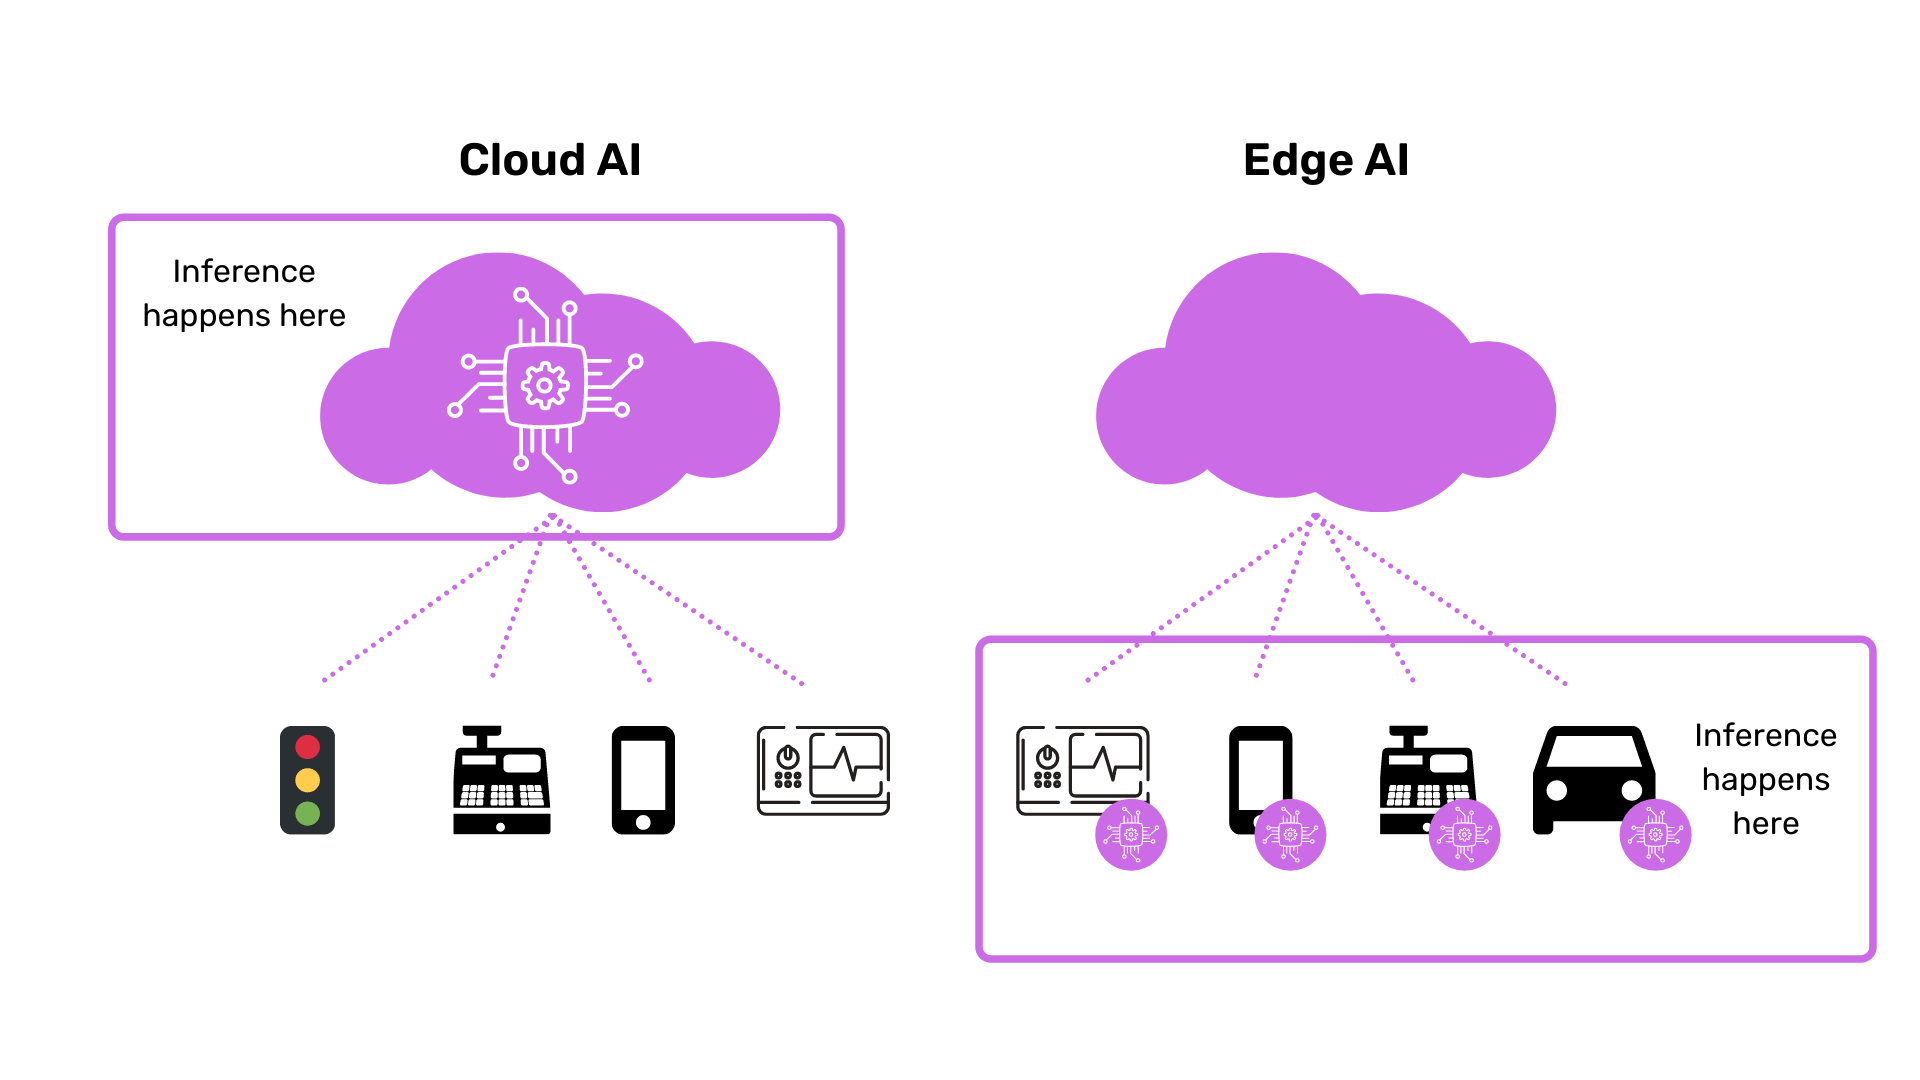
\includegraphics[width=0.6\textwidth]{image/CloudAIvsEdgeAI-1920w.png}
    \caption{Cloud AI và Edge AI}
    \label{fig:cloud_edge_ai}
\end{figure}

Trong đề tài này, Edge AI được triển khai như một module phân tích dữ liệu chuỗi thời gian (Time Series), đảm nhiệm chức năng dự báo sớm nồng độ bụi mịn PM2.5 dựa trên các thông số môi trường thực tế ngay tại hiện trường.

\subsection{Tổng quan mô hình TCN (Temporal Convolutional Network) và lý do lựa chọn TCN}

\subsubsection{Tổng quan về kiến trúc TCN}

Temporal Convolutional Network (TCN) là một kiến trúc mạng nơ-ron được thiết kế chuyên biệt cho bài toán xử lý dữ liệu chuỗi thời gian. Mô hình này kết hợp ưu điểm của mạng tích chập (Convolutional Neural Network -- CNN) với khả năng học các phụ thuộc dài hạn tương tự như mạng hồi tiếp (Recurrent Neural Network -- RNN) \cite{li2023_tcn_bilstm_dmattention,wang2024_causal_stan}.

\begin{figure}[H]
    \centering
    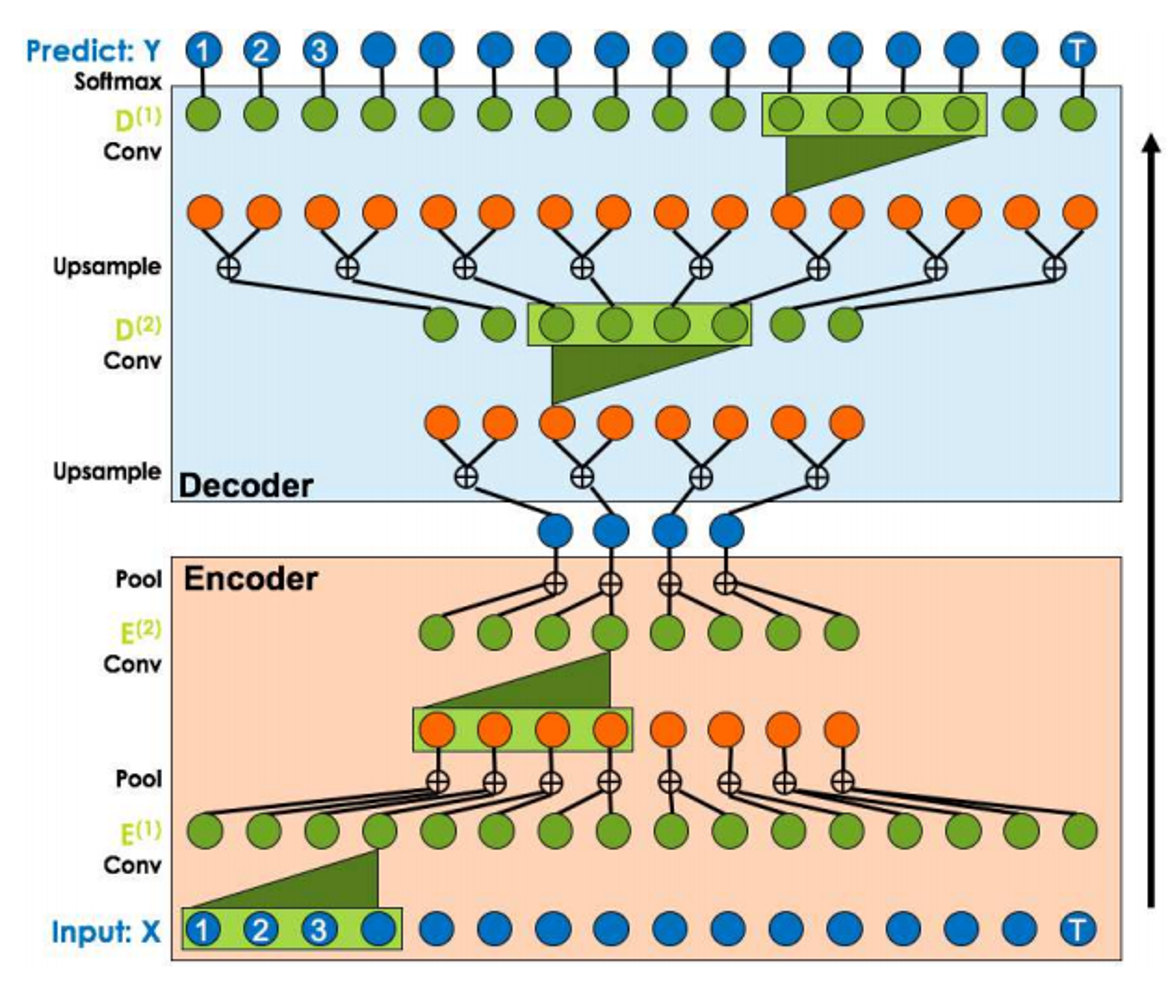
\includegraphics[width=0.5\textwidth]{image/TCN.png}
    \caption{Kiến trúc mô hình TCN}
    \label{fig:tcn_architecture}
\end{figure}

Kiến trúc TCN được xây dựng dựa trên hai nguyên lý cốt lõi:

\begin{itemize}
    \item \textbf{Causal Convolution (Tích chập nhân quả):}
    Đảm bảo rằng tại thời điểm $t$, mô hình chỉ sử dụng các thông tin từ các thời điểm trước đó và hiện tại, tức là từ $0$ đến $t$. Điều này giúp ngăn chặn hiện tượng ``rò rỉ'' thông tin từ tương lai vào quá trình dự báo.

    \item \textbf{Dilated Convolution (Tích chập giãn cách):}
    Các phần tử trong bộ lọc được áp dụng với khoảng cách giãn $d$, giúp mở rộng trường thụ cảm (\textit{receptive field}) theo cấp số nhân mà không làm tăng đáng kể số lượng tham số của mô hình.
\end{itemize}

Trong đề tài này, mô hình được cấu hình với các hệ số giãn cách:
\[
d = \{1, 2, 4, 8\}
\]

Cấu hình này cho phép mô hình quan sát hiệu quả các biến động của nồng độ bụi mịn PM2.5 trong khoảng thời gian 30 phút trước đó, từ đó nâng cao khả năng dự báo cho các bước thời gian tiếp theo.

\subsubsection{Lý do lựa chọn TCN thay vì LSTM/RNN}

Sau quá trình thực nghiệm và tối ưu hóa cho hệ thống Edge AI, trong luận văn nhóm đã lựa chọn kiến trúc TCN thay thế cho các mô hình LSTM và RNN nhờ nhiều ưu điểm về hiệu năng và khả năng triển khai trên thiết bị nhúng. Khác với RNN và LSTM phải xử lý dữ liệu tuần tự theo từng bước thời gian, TCN sử dụng phép tích chập trên toàn bộ chuỗi dữ liệu, cho phép tận dụng khả năng tính toán song song của phần cứng nhằm giảm đáng kể thời gian huấn luyện và suy luận. Ngoài ra, cấu trúc tích chập phân tầng kết hợp với residual connection giúp TCN giảm hiện tượng mất mát đạo hàm và học ổn định hơn khi xử lý các phụ thuộc dài hạn trong chuỗi thời gian.

Bên cạnh đó, TCN cho phép điều chỉnh linh hoạt trường thụ cảm thông qua các tham số như \texttt{kernel\_size} và \texttt{dilations}, giúp kiểm soát hiệu quả độ dài chuỗi dữ liệu được sử dụng để dự báo. Nhiều nghiên cứu gần đây cũng cho thấy TCN đạt hiệu quả cao trong các bài toán dự báo chất lượng không khí và nồng độ PM2.5 \cite{li2023_tcn_bilstm_dmattention,wang2024_causal_stan,stoten2025_pm25}. Ngoài hiệu quả dự báo, kiến trúc TCN còn có cấu trúc gọn nhẹ, số lượng tham số thấp và dễ dàng chuyển đổi sang định dạng TensorFlow Lite Float16. Trong đề tài này, mô hình sau khi lượng tử hóa đã giảm khoảng 50\% dung lượng lưu trữ nhưng vẫn duy trì độ chính xác dự báo ở mức cao, phù hợp để triển khai trên các thiết bị Edge AI như Raspberry Pi 4.

\subsection{Định dạng mô hình trung gian và tối ưu hóa trên thiết bị Edge}

\subsubsection{Định dạng mô hình ONNX (Open Neural Network Exchange)}

ONNX (Open Neural Network Exchange) là một định dạng mở được thiết kế để biểu diễn các mô hình học máy, cho phép chuyển đổi linh hoạt giữa nhiều framework khác nhau như PyTorch, TensorFlow và Keras.

\begin{figure}[H]
    \centering
    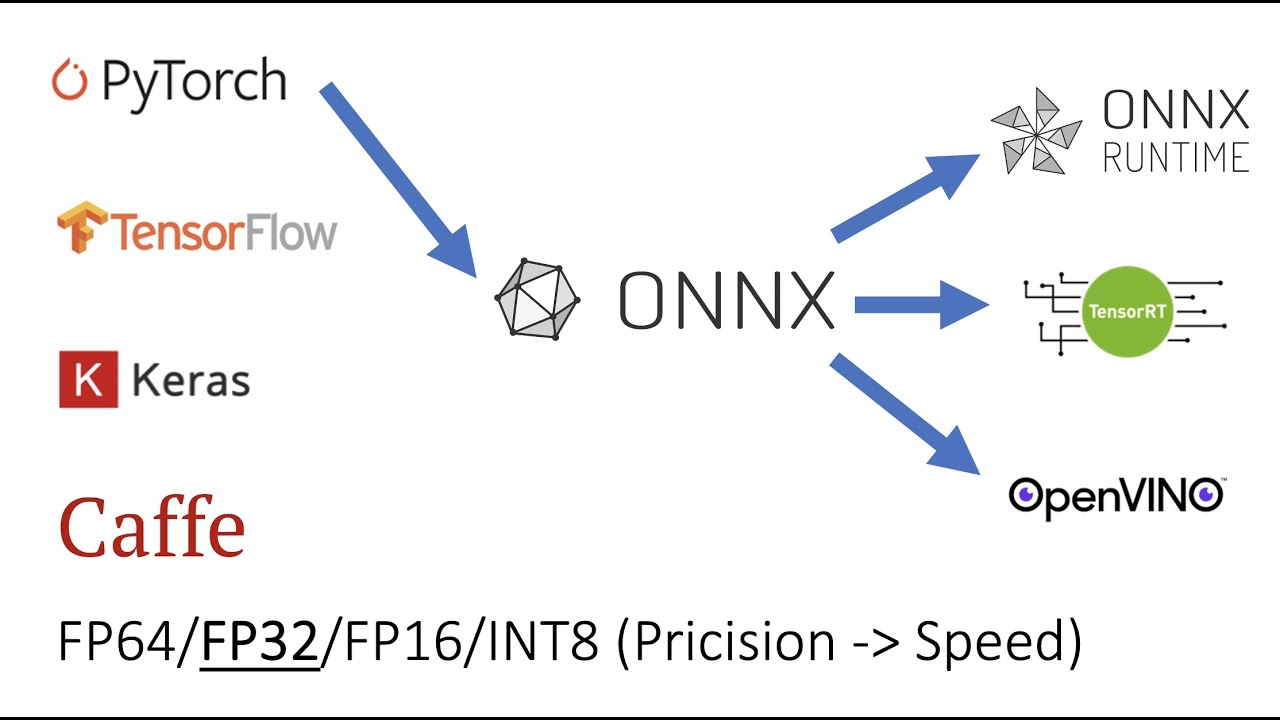
\includegraphics[width=0.6\textwidth]{image/ONNX.jpg}
    \caption{Định dạng ONNX}
    \label{fig:onnx}
\end{figure}

Trong đề tài này, ONNX đóng vai trò như một ``ngôn ngữ chung'' cho mô hình học sâu. Việc chuyển đổi mô hình sang định dạng ONNX giúp hệ thống có thể tận dụng các công cụ tối ưu hóa và các bộ tăng tốc phần cứng khác nhau mà không phụ thuộc vào môi trường huấn luyện ban đầu.

Một ưu điểm quan trọng của ONNX là khả năng tối ưu hóa đồ thị tính toán (\textit{graph optimization}), bao gồm việc loại bỏ các nút dư thừa, hợp nhất các phép toán liên tiếp và đơn giản hóa cấu trúc mô hình nhằm cải thiện tốc độ suy luận.

\subsubsection{Định dạng TensorFlow Lite (TFLite) và tối ưu hóa Float16}

TensorFlow Lite (TFLite) là thư viện mã nguồn mở được phát triển nhằm tối ưu hóa quá trình suy luận (\textit{inference}) trên các thiết bị di động và hệ thống nhúng có tài nguyên phần cứng hạn chế.

\begin{figure}[H]
    \centering
    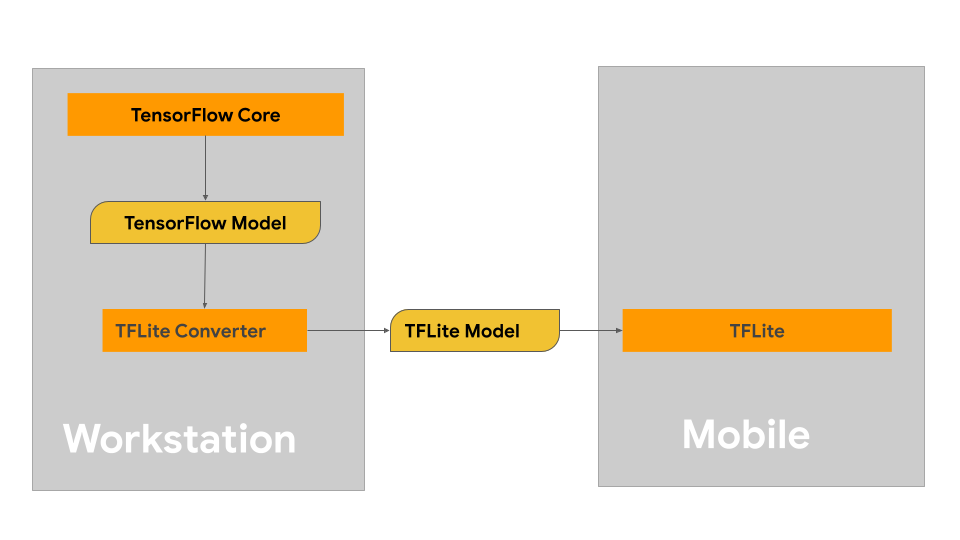
\includegraphics[width=0.6\textwidth]{image/TFLITE.png}
    \caption{Định dạng TensorFlow Lite}
    \label{fig:tflite}
\end{figure}

Trong hệ thống được xây dựng, kỹ thuật \textit{Float16 Quantization} được áp dụng trong quá trình chuyển đổi mô hình (thực hiện trong file \texttt{convert.py}). Cụ thể, các trọng số của mô hình được chuyển từ định dạng số thực dấu phẩy động 32-bit (Float32) sang 16-bit (Float16).

Việc lượng tử hóa Float16 mang lại các lợi ích sau:

\begin{itemize}
    \item \textbf{Giảm dung lượng mô hình:}
    Kích thước tệp mô hình giảm khoảng 50\% so với mô hình gốc, giúp tiết kiệm bộ nhớ lưu trữ trên thiết bị nhúng.

    \item \textbf{Tăng tốc độ suy luận:}
    Nhiều bộ xử lý hiện đại hỗ trợ tính toán Float16 hiệu quả, giúp giảm độ trễ (\textit{latency}) khi dự báo chỉ số PM2.5 theo thời gian thực.

    \item \textbf{Duy trì độ chính xác cao:}
    So với lượng tử hóa Int8, định dạng Float16 thường giữ được độ chính xác gần như tương đương với mô hình gốc, đồng thời ít gây sai lệch kết quả dự báo.
\end{itemize}

\section{Giao tiếp phần cứng công nghiệp}
\subsection{Chuẩn vật lý RS485}
\begin{figure}[H]
    \centering
    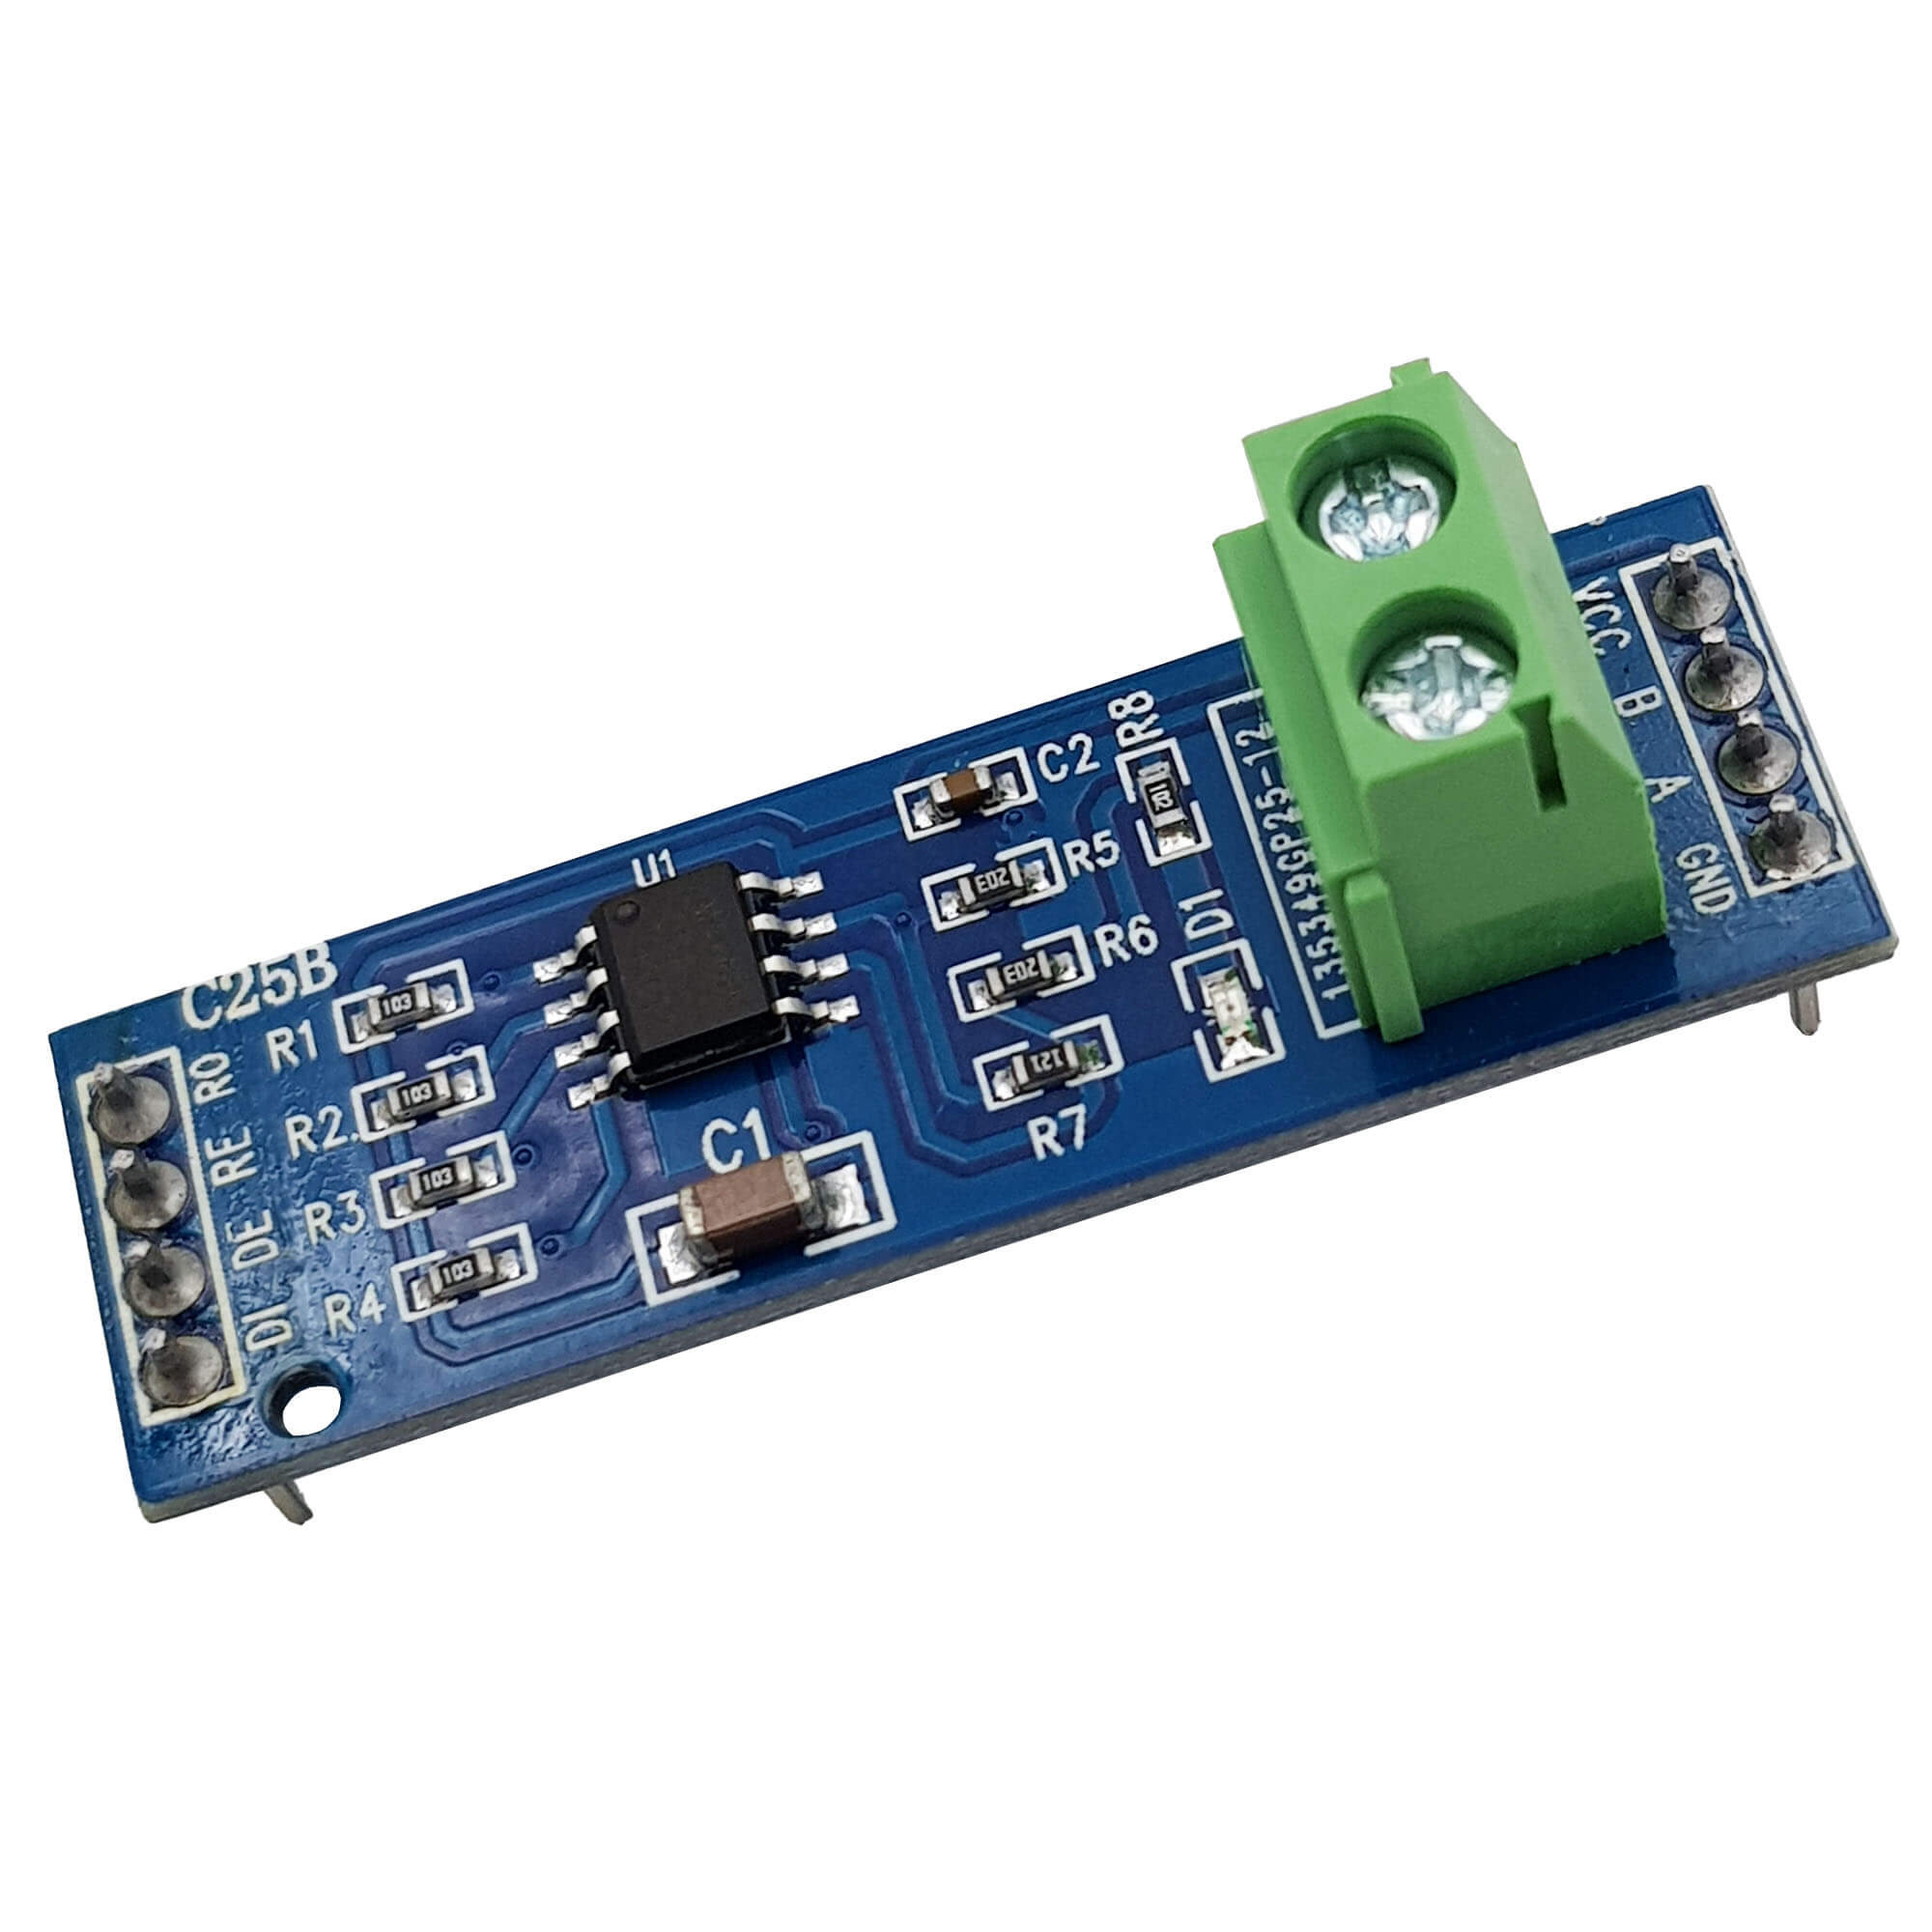
\includegraphics[width=0.2\linewidth]{image/rs485.jpg}
    \caption{RS485 TTL }
    \label{fig:placeholder}
\end{figure}
Chuẩn RS485 (Recommended Standard 485) là một chuẩn truyền thông ở tầng vật lý, được Hiệp hội Công nghiệp Điện tử (EIA) ban hành nhằm phục vụ các hệ thống truyền dữ liệu nối tiếp trong môi trường công nghiệp. RS485 được thiết kế để đáp ứng yêu cầu truyền dữ liệu ổn định trên khoảng cách xa, chống nhiễu tốt và hỗ trợ nhiều thiết bị cùng kết nối trên một đường truyền, do đó được sử dụng rộng rãi trong các hệ thống điều khiển, giám sát và tự động hóa công nghiệp.


Về mặt nguyên lý hoạt động, RS485 sử dụng phương pháp truyền tín hiệu vi sai (differential signaling) thông qua hai dây tín hiệu A và tín hiệu B. Dữ liệu được biểu diễn bằng sự chênh lệch điện áp giữa hai dây này thay vì so với mass (hoặc GND) như các chuẩn truyền đơn cực. Cách truyền vi sai giúp RS485 có khả năng chống nhiễu điện từ cao, đặc biệt phù hợp với môi trường công nghiệp nơi tồn tại nhiều nguồn nhiễu như động cơ, biến tần và thiết bị công suất lớn.

Nhờ các đặc tính nổi bật như khả năng truyền xa, chống nhiễu tốt, hỗ trợ nhiều thiết bị và chi phí triển khai thấp, chuẩn RS485 vẫn giữ vai trò quan trọng trong các hệ thống công nghiệp hiện đại. Mặc dù đã xuất hiện nhiều chuẩn truyền thông mới, RS485 vẫn là lựa chọn ưu tiên trong các ứng dụng yêu cầu độ tin cậy cao, cấu trúc đơn giản và khả năng hoạt động ổn định trong môi trường khắc nghiệt.

Trong hệ thống IoT và Linux Embedded, RS485 thường được kết hợp với các giao thức truyền thông công nghiệp như Modbus RTU nhằm hỗ trợ trao đổi dữ liệu giữa gateway và các cảm biến hoặc thiết bị điều khiển.
\subsection{Giao thức Modbus RTU và cấu trúc khung tin}
\subsubsection{Giao thức Modbus RTU}


Modbus RTU (Remote Terminal Unit) là một giao thức truyền thông công nghiệp phổ biến, được phát triển bởi Modicon vào năm 1979. Đây là giao thức dạng master–slave (hiện nay còn gọi là client–server), được thiết kế nhằm cho phép các thiết bị điều khiển và giám sát trong công nghiệp trao đổi dữ liệu với nhau một cách đơn giản, tin cậy và hiệu quả. Nhờ tính mở, dễ triển khai và khả năng tương thích cao, Modbus RTU hiện vẫn được sử dụng rộng rãi trong các hệ thống SCADA, PLC, cảm biến và thiết bị đo lường công nghiệp.

Trong mô hình hoạt động của Modbus RTU, thiết bị master đóng vai trò khởi tạo và điều khiển toàn bộ quá trình truyền thông, trong khi các thiết bị slave chỉ phản hồi khi nhận được yêu cầu hợp lệ từ master. Mỗi thiết bị slave được gán một địa chỉ duy nhất trên bus, giúp master xác định đúng thiết bị cần giao tiếp. Cơ chế này giúp tránh xung đột dữ liệu và đảm bảo tính tuần tự trong quá trình truyền thông.


\subsubsection{Cấu trúc khung tin}


Modbus RTU truyền dữ liệu dưới dạng các khung tin (frame) được mã hóa theo dạng nhị phân, cho phép tiết kiệm băng thông và nâng cao hiệu quả truyền thông. Mỗi khung tin Modbus RTU bao gồm các trường dữ liệu được sắp xếp theo thứ tự xác định, đảm bảo thiết bị nhận có thể giải mã chính xác nội dung thông tin.


Một khung tin Modbus RTU tiêu chuẩn bao gồm các thành phần chính: địa chỉ thiết bị, mã hàm, vùng dữ liệu và mã kiểm tra lỗi CRC. Khung tin được phân tách với các khung khác bằng một khoảng im lặng trên đường truyền (silent interval), có độ dài tối thiểu tương đương 3.5 ký tự, giúp thiết bị nhận xác định ranh giới giữa các khung dữ liệu.


Trường địa chỉ thiết bị có độ dài 1 byte, dùng để xác định slave mà master muốn giao tiếp. Địa chỉ hợp lệ nằm trong khoảng từ 1 đến 247, trong khi địa chỉ 0 được sử dụng cho chế độ broadcast, cho phép master gửi lệnh đến tất cả các slave mà không yêu cầu phản hồi.


Mỗi khung tin Modbus RTU kết thúc bằng trường CRC (Cyclic Redundancy Check) dài 2 byte. CRC được sử dụng để kiểm tra lỗi trong quá trình truyền dữ liệu, giúp phát hiện các lỗi do nhiễu hoặc sai lệch tín hiệu trên đường truyền. Slave hoặc master sẽ tự động tính toán CRC của khung tin nhận được và so sánh với giá trị CRC đi kèm để xác định tính toàn vẹn của dữ liệu.


Mặc dù đã xuất hiện nhiều giao thức truyền thông công nghiệp hiện đại hơn, Modbus RTU vẫn giữ vai trò quan trọng trong thực tế nhờ độ ổn định, tính phổ biến và khả năng tương thích rộng rãi. Việc hiểu rõ nguyên lý hoạt động và cấu trúc khung tin Modbus RTU là nền tảng quan trọng cho việc thiết kế, triển khai và vận hành các hệ thống giám sát và điều khiển công nghiệp.

\section{Kết nối Cloud và IoT}
\subsection{Tổng quan về CoreIOT}

\begin{figure}[H]
    \centering
    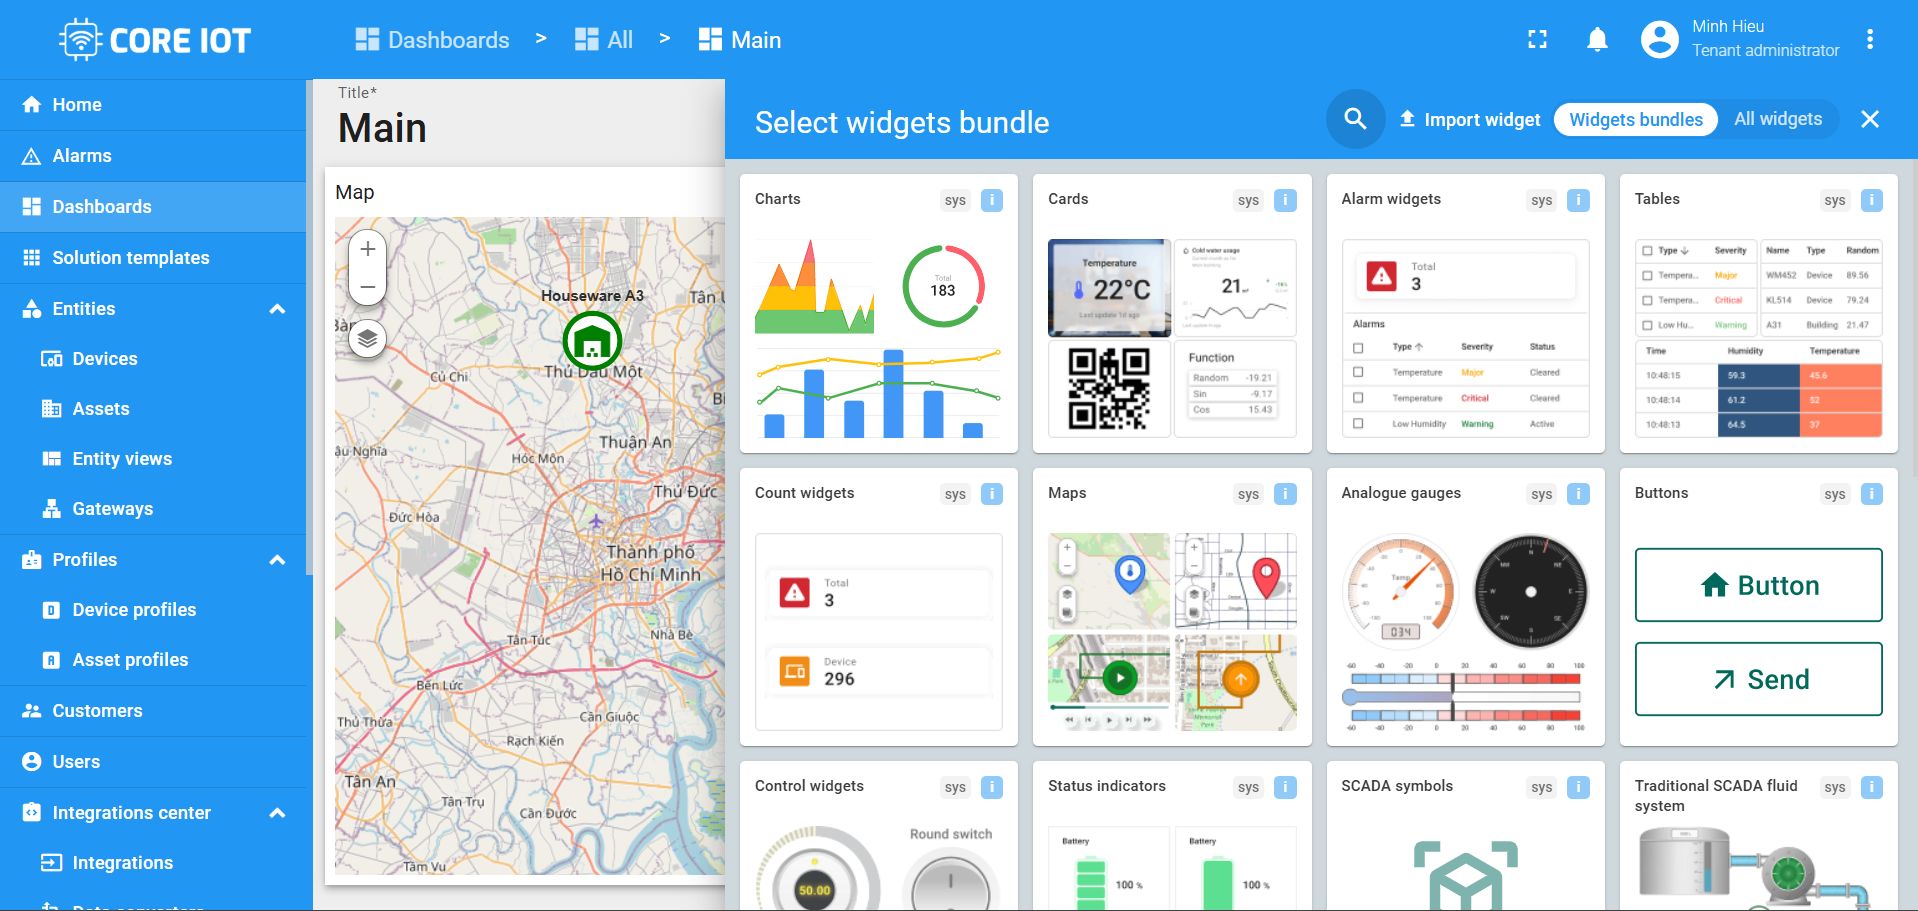
\includegraphics[width=1\textwidth]{image/coreiotp.png}
    \caption{Tổng quan về CoreIOT}
    \label{fig:coreiot}
\end{figure}

CoreIoT là một nền tảng Internet of Things (IoT) được phát triển và xây
dựng dựa trên định hướng tương tự các nền tảng IoT mã nguồn mở phổ biến như
ThingsBoard, nhằm phục vụ nhu cầu giảng dạy, nghiên cứu và triển khai các bài
toán IoT trong môi trường học thuật và đào tạo kỹ thuật. Nền tảng được tùy
biến và phát triển lại để phù hợp với điều kiện sử dụng, ngôn ngữ và đối tượng
người dùng là sinh viên, giảng viên và các nhóm nghiên cứu tại nhà trường.

Về mặt kiến trúc tổng thể, CoreIoT được thiết kế theo mô hình nền tảng trung
tâm, cho phép thu thập, xử lý, lưu trữ và hiển thị dữ liệu từ các thiết bị IoT
phân tán. Hệ thống đóng vai trò trung gian giữa các thiết bị đầu cuối và người
dùng, hỗ trợ quản lý thiết bị, giám sát dữ liệu theo thời gian thực và xây dựng
các ứng dụng IoT hoàn chỉnh. Cách tiếp cận này giúp người học dễ dàng tiếp cận
các khái niệm cốt lõi của IoT mà không cần triển khai toàn bộ hạ tầng từ đầu.

CoreIoT hỗ trợ kết nối với các thiết bị IoT thông qua các giao thức truyền
thông phổ biến, đặc biệt phù hợp với các thiết bị nhúng và hệ thống công nghiệp.
Dữ liệu từ cảm biến sau khi được thu thập tại thiết bị biên sẽ được truyền về
nền tảng để xử lý và lưu trữ tập trung. Thông qua đó, CoreIoT cho phép theo
dõi trạng thái thiết bị, phân tích dữ liệu và hiển thị thông tin trực quan trên
dashboard, hỗ trợ người dùng giám sát hệ thống một cách hiệu quả.

Bên cạnh chức năng giám sát, CoreIoT còn hỗ trợ xây dựng các quy tắc xử lý
dữ liệu và sự kiện thông qua cơ chế xử lý logic ở tầng nền tảng. Các quy tắc này
cho phép hệ thống phản ứng tự động trước các điều kiện cụ thể, chẳng hạn như
phát cảnh báo khi giá trị cảm biến vượt ngưỡng hoặc ghi nhận sự kiện phục vụ
phân tích sau này. Cách tiếp cận này giúp người học hiểu rõ hơn về mô hình xử
lý dữ liệu và tự động hóa trong các hệ thống IoT hiện đại.

Với định hướng phục vụ đào tạo và nghiên cứu, CoreIoT không chỉ đóng vai
trò là một công cụ giám sát mà còn là môi trường thực hành giúp sinh viên tiếp
cận các khái niệm quan trọng như quản lý thiết bị, truyền thông IoT, xử lý dữliệu thời gian thực và tích hợp hệ thống. Nền tảng tạo điều kiện thuận lợi cho
việc triển khai các đề tài học tập, đồ án và nghiên cứu ứng dụng, đồng thời có
khả năng mở rộng để đáp ứng các bài toán IoT phức tạp hơn trong tương lai.


\subsection{Giao thức MQTT trong hệ thống nhúng}
\begin{figure}[!h]
    \centering
    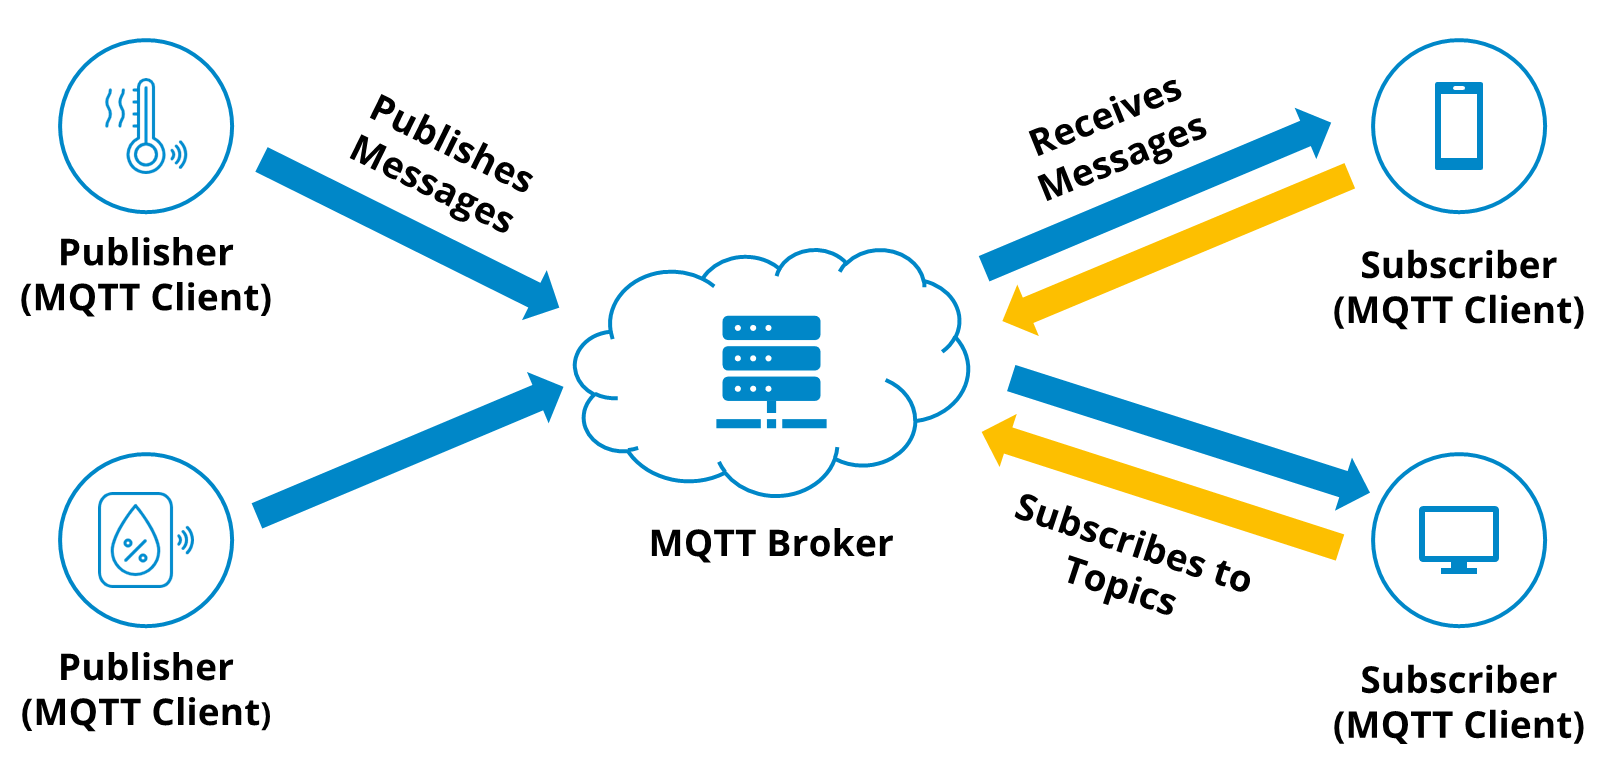
\includegraphics[width=0.6\textwidth]{image/mqtt1.png}
    \caption{Giao thức MQTT trong hệ thống nhúng}
    \label{fig:mqtt}

\end{figure}

MQTT (Message Queuing Telemetry Transport) là một giao thức truyền tin
nhẹ, được thiết kế theo mô hình publish–subscribe, đặc biệt phù hợp cho các
hệ thống IoT có tài nguyên hạn chế và yêu cầu truyền dữ liệu với độ trễ thấp.
Trong mô hình này, các thiết bị không giao tiếp trực tiếp với nhau mà thông
qua một thành phần trung gian gọi là broker. Thiết bị gửi dữ liệu sẽ đóng vai
trò publisher, trong khi thiết bị nhận dữ liệu là subscriber, và broker chịu trách
nhiệm phân phối thông điệp dựa trên các chủ đề (topic).

Một đặc điểm nổi bật của MQTT là kích thước gói tin nhỏ, giúp giảm băng thông và tiết kiệm năng lượng, rất phù hợp với các thiết bị nhúng và mạng truyền
thông không ổn định. MQTT hỗ trợ nhiều mức chất lượng dịch vụ (Quality of
Service – QoS), cho phép cân bằng giữa độ tin cậy và hiệu năng truyền thông.
Bên cạnh đó, giao thức còn hỗ trợ cơ chế giữ kết nối (keep-alive), thông báo trạng
thái thiết bị và khả năng mở rộng linh hoạt trong các hệ thống IoT quy mô lớn.
Nhờ các đặc tính trên, MQTT thường được sử dụng trong các ứng dụng giám
sát thời gian thực, thu thập dữ liệu cảm biến, hệ thống điều khiển từ xa và các
nền tảng IoT trung tâm như CoreIoT hoặc các nền tảng tương đương.

